\documentclass[a4paper,12pt]{article}
\usepackage[utf8]{inputenc} 
\usepackage{amsmath}
\usepackage{xcolor}
\usepackage{graphicx}
\usepackage[citecolor=blue]{hyperref}       % Para enlaces en el documento
\usepackage{fancyhdr}
\usepackage{circuitikz}
\usepackage{amssymb}
\usepackage{animate}
\usepackage{float}
\usepackage{multirow}
\usepackage{pgfplots}
\pgfplotsset{compat=1.18}
\usepackage[a4paper, margin=1in]{geometry}
\usepackage{gensymb}
\usepackage{siunitx}
\usepackage{booktabs}
\usepackage{array}
\usepackage{tabularx}
\usepackage{listings}
\usepackage{tikz}
\usetikzlibrary{shapes.geometric, arrows, positioning}

% Ajuste de la altura del encabezado
\setlength{\headheight}{76.27646pt}
\addtolength{\topmargin}{-34.27646pt}

\lstdefinestyle{mystyle}{
    language=Matlab,
    inputencoding=utf8,
    backgroundcolor=\color{black!5},
    commentstyle=\color{green!60!black},
    keywordstyle=\color{blue},
    numberstyle=\tiny\color{gray},
    stringstyle=\color{purple},
    basicstyle=\footnotesize\ttfamily,
    breaklines=true,
    captionpos=b,
    keepspaces=true,
    numbers=left,
    numbersep=5pt,
    showstringspaces=false,
}
\lstset{style=mystyle}

\setlength{\parindent}{0pt}

% Crear la portada manualmente
\begin{document}

% Desactivar la numeración de página para la portada
\thispagestyle{empty}

% Colocar las imágenes en las esquinas superiores
\begin{minipage}[t]{0.4\textwidth}
    \raggedright
    
\includegraphics[width=2cm]{image/der.png}
\end{minipage}%
\begin{minipage}[t]{0.5\textwidth}
    \raggedleft
    
\includegraphics[width=2cm]{image/izq.png}
\end{minipage}

\vspace{1cm}

\begin{center}
    \Huge{\textbf{Previo 6}} \\
    \vspace{0.5cm}
    \LARGE{\textbf{Encaminamiento y análisis de paquetes.}} \\
    \vspace{0.5cm}
    \Large{\textbf{Cuestionario Previo}} \\
    \vspace{1cm}
    \Large{\textbf{Universidad Nacional Autónoma de México.}}\\
    \Large{\textbf{Facultad de Ingeniería.}}\\
    \vspace{1cm}
    \Large{Laboratorio de Redes de datos seguras.} \\
    \vspace{0.5cm}
    \LARGE{\textbf{Profesora:}}
    \LARGE{\textit{MTRA. MARÍA EUGENIA BAUTISTA GONZÁLEZ.}}\\
    \vspace{0.5cm}
    \Large{\textbf{Grupo:} 08} \\
    \vspace{0.5cm}
    \LARGE{\textbf{Alumno:}}\\
    \Large{320060829} \\
    \vspace{3cm}
    \Large{\textbf{Fecha de Entrega:}}\\
    \vspace{0.5cm}
    \large{{19 de Marzo de 2026}}
\end{center} 


\newpage

% Configuración del encabezado y pie de página
\pagestyle{fancy}
\fancyhf{}
\fancyhead[L]{
\includegraphics[width=1.5cm]{image/der.png}}
\fancyhead[R]{
\includegraphics[width=1.5cm]{image/izq.png}}
\fancyfoot[C]{\thepage}  % Coloca el número de página en el centro del pie de página

% Línea horizontal en el pie de página
\renewcommand{\footrulewidth}{0.4pt}  % Define el grosor de la línea en el pie de página

% Empezar numeración de páginas desde 1 en la segunda página
\pagenumbering{arabic}
\setcounter{page}{1}

%\maketitle
\tableofcontents


\newpage

\section{Describa las funciones de la capa 3 (capa de red) del Modelo OSI}

El Modelo de Interconexión de Sistemas Abiertos (OSI), estandarizado por la Organización Internacional de Normalización, divide la arquitectura de las comunicaciones de red en siete capas abstractas, proporcionando un marco de referencia universal para la interoperabilidad entre sistemas heterogéneos. Dentro de este paradigma, la Capa 3, comúnmente denominada capa de red, asume la responsabilidad crítica de gobernar el tránsito de la información desde un host de origen hasta un host de destino final a través de múltiples redes interconectadas, independientemente de la topología física o los medios de transmisión subyacentes. A diferencia de la capa de enlace de datos (Capa 2), que se circunscribe a la entrega de tramas dentro de un mismo segmento de red local o dominio de difusión, la capa de red implementa un esquema de direccionamiento lógico jerárquico que permite la escalabilidad global de las comunicaciones.

La primera función medular de la capa de red es el direccionamiento lógico. Mientras que las direcciones físicas (como las direcciones MAC) son planas y están grabadas en el hardware, careciendo de información topológica, el direccionamiento lógico proporciona una estructura jerárquica. En el ecosistema dominante actual, esta función es ejecutada casi en su totalidad por el Protocolo de Internet (IP), tanto en su versión 4 (IPv4) como en la versión 6 (IPv6). Una dirección IP no solo identifica de forma unívoca a un nodo específico en la internetwork, sino que también, mediante el uso de máscaras de subred, delimita matemáticamente a qué red o subred pertenece dicho nodo. Esta dualidad estructural es el pilar que permite a los dispositivos intermediarios, como los enrutadores, tomar decisiones de reenvío basadas en grupos de direcciones (redes) en lugar de tener que procesar la ubicación individual de miles de millones de dispositivos finales.

La segunda función primordial es el encapsulamiento. Cuando los protocolos de la capa de transporte (Capa 4), como el Protocolo de Control de Transmisión (TCP) o el Protocolo de Datagramas de Usuario (UDP), transfieren sus segmentos o datagramas hacia abajo en la pila del modelo OSI, la capa de red los recibe y los encapsula agregando un encabezado específico de Capa 3. Este nuevo constructo de datos se denomina paquete. El encabezado IP adjunto contiene parámetros de control vitales, siendo los más significativos las direcciones lógicas de origen y destino. Es imperativo comprender que, a diferencia de los encabezados de la Capa 2 que son reescritos en cada salto físico que da la información, las direcciones de origen y destino en el encabezado de la Capa 3 permanecen conceptualmente inmutables durante todo el trayecto desde el emisor hasta el receptor final, salvo en escenarios donde se aplican tecnologías de Traducción de Direcciones de Red (NAT) en los perímetros de las redes corporativas.

La tercera y más compleja de las funciones es el encaminamiento o enrutamiento. Dado que las redes modernas están formadas por múltiples rutas convergentes y divergentes, los paquetes rara vez viajan en una línea recta de origen a destino. Los enrutadores son los dispositivos de red especializados que operan en esta capa, encargados de inspeccionar la dirección IP de destino de cada paquete entrante y consultar sus tablas de enrutamiento internas. Estas tablas, construidas estáticamente por administradores o dinámicamente mediante algoritmos matemáticos complejos, dictaminan cuál es la interfaz de salida óptima o el router del "próximo salto" (next-hop) al que se debe transferir el paquete para acercarlo a su destino final. Este proceso de toma de decisiones se realiza paquete por paquete y salto por salto, garantizando que los datos puedan sortear enlaces congestionados o caídos.

Finalmente, la capa de red es responsable del proceso de desencapsulamiento. Una vez que un paquete ha navegado exitosamente por la internetwork y llega a la interfaz de red del dispositivo de destino final, este host verifica la dirección IP del paquete. Si la dirección de destino coincide exactamente con la dirección lógica configurada en su propia interfaz (o es una dirección de difusión/multidifusión que el host está programado para aceptar), la capa de red procede a eliminar el encabezado IP. Tras esta eliminación, la unidad de datos de protocolo (PDU) subyacente de la Capa 4 es expuesta y transferida hacia los niveles superiores para su procesamiento aplicativo. Desde el punto de vista de las redes de datos seguras, la comprensión exhaustiva de estas cuatro funciones es indispensable, ya que vectores de ataque críticos como la suplantación de IP (IP Spoofing), los ataques de denegación de servicio distribuido (DDoS) mediante fragmentación o inundación ICMP, y el secuestro de rutas (Route Hijacking) explotan directamente las mecánicas operativas y la falta de autenticación inherente en el diseño original de la capa de red.

\section{¿Cuáles son los principales campos que forman la trama Ethernet?}

Para que un paquete de la capa de red pueda ser transmitido físicamente a través de un medio de red local, como un cable de cobre de par trenzado o un enlace de fibra óptica, debe descender a la Capa 2 del Modelo OSI (Capa de Enlace de Datos) para su encapsulamiento final antes de la transmisión eléctrica u óptica. En la inmensa mayoría de las redes de área local (LAN) contemporáneas, el protocolo dominante en esta capa es Ethernet, estandarizado bajo la familia de normas IEEE 802.3. Ethernet opera fragmentando el flujo de datos en unidades discretas denominadas tramas (frames). La trama no solo transporta el paquete de datos, sino que proporciona los mecanismos de control necesarios para el acceso al medio compartido, el direccionamiento físico y la detección de errores de transmisión. El formato más extendido y utilizado en la actualidad es la trama Ethernet II (también conocida como formato DIX), cuya longitud total debe oscilar estrictamente entre un mínimo de 64 bytes y un máximo de 1518 bytes (excluyendo el preámbulo).

La anatomía de una trama Ethernet II es altamente estructurada y se compone de campos binarios secuenciales que los controladores de interfaz de red (NIC) y los conmutadores (switches) interpretan a velocidades de nanosegundos. A continuación, se presenta una tabla detallada con los campos principales que conforman esta trama, seguida de un análisis técnico de su propósito operativo y sus implicaciones en redes seguras.

\begin{table}[H]
\centering
\caption{Estructura y campos principales de la trama Ethernet II}
\vspace{0.3cm}
\footnotesize
\begin{tabularx}{\linewidth}{@{}>{\raggedright\arraybackslash}p{4.1cm}>{\centering\arraybackslash}p{2.2cm}>{\raggedright\arraybackslash}X@{}}
\toprule
\textbf{Campo de la Trama} & \textbf{Tamaño} & \textbf{Descripción Técnica} \\ \midrule
Preámbulo & 7 bytes & Secuencia de bits (10101010) para sincronización de reloj. \\
Delimitador de Inicio (SFD) & 1 byte & Patrón (10101011) que marca el inicio de la trama lógica. \\
MAC de Destino & 6 bytes & Dirección física del hardware receptor en la red local. \\
MAC de Origen & 6 bytes & Dirección física del hardware emisor de la trama. \\
EtherType (Tipo) & 2 bytes & Identificador del protocolo de capa de red encapsulado. \\
Datos (Carga Útil / Payload) & 46 - 1500 bytes & El paquete IP o PDU de Capa 3. Incluye relleno si es necesario. \\
Secuencia de Verificación (FCS)& 4 bytes & Valor CRC-32 para la detección de errores físicos en tránsito. \\ \bottomrule
\end{tabularx}
\end{table}

El primer componente que viaja por el medio físico es el Preámbulo, un bloque de 7 bytes que consiste en un patrón binario alternante de unos y ceros (10101010). Su función exclusiva es "despertar" a los circuitos receptores y permitir que los relojes de las tarjetas de red se sincronicen con la temporización de la señal eléctrica entrante. Inmediatamente después, el Delimitador de Inicio de Trama (Start Frame Delimiter o SFD) utiliza un byte específico (10101011) cuyo último bit, al romper la alternancia y presentar dos unos consecutivos, le indica categóricamente a la tarjeta de red que la sincronización ha concluido y que los siguientes bits constituyen el inicio oficial de la cabecera de la trama lógica con información de direccionamiento.

A continuación, se encuentran los campos de direccionamiento de control de acceso al medio (MAC). La Dirección MAC de Destino, de 6 bytes de longitud, identifica el nodo o nodos que deben procesar la trama dentro del segmento local. Esta dirección puede representar una transmisión de unidifusión (dirigida a un solo dispositivo), multidifusión (a un grupo específico) o difusión (broadcast, representada hexadecimalmente como FF:FF:FF:FF:FF:FF, que obliga a todos los dispositivos en el dominio de colisión a procesar la trama). Posteriormente se ubica la Dirección MAC de Origen, también de 6 bytes, que siempre es una dirección de unidifusión correspondiente a la interfaz de hardware que está inyectando la trama en el medio. En el ámbito de la ciberseguridad, estos campos son frecuentemente manipulados. Los atacantes utilizan técnicas de suplantación de identidad (MAC Spoofing) para eludir listas de control de acceso basadas en MAC, o realizan ataques de inundación de direcciones MAC (MAC Flooding) para desbordar la tabla de memoria de contenido direccionable (CAM) de un switch corporativo, forzándolo a operar como un hub y permitiendo la interceptación del tráfico ajeno.

El campo EtherType, de 2 bytes, actúa como un elemento multiplexor. Le indica a la capa de enlace de datos a qué protocolo de red de la capa superior debe entregarle la carga útil una vez que la trama ha sido procesada exitosamente. Por ejemplo, un valor hexadecimal de 0x0800 especifica que el contenido es un paquete IPv4, mientras que un valor de 0x0806 indica que la trama transporta un mensaje del Protocolo de Resolución de Direcciones (ARP). 

El campo de Datos, también conocido como carga útil o payload, contiene el paquete de la Capa 3 completamente encapsulado. Las especificaciones del estándar Ethernet dictan que este campo debe tener un tamaño mínimo de 46 bytes para asegurar que las tramas sean lo suficientemente largas como para que el mecanismo de detección de colisiones CSMA/CD funcione correctamente a través de la longitud máxima del cableado. Si el paquete IP subyacente es menor a 46 bytes, la tarjeta de red del emisor insertará ceros adicionales, conocidos como bits de relleno (padding), hasta alcanzar el mínimo requerido. El tamaño máximo estándar de este campo es de 1500 bytes, lo que se conoce como la Unidad Máxima de Transferencia (MTU).

Finalmente, la trama se cierra con la Secuencia de Verificación de Trama (Frame Check Sequence o FCS), un campo de 4 bytes fundamental para la integridad de los datos. Antes de enviar la trama, el hardware emisor procesa todos los campos desde la MAC de destino hasta el final de los datos a través de un complejo algoritmo de polinomio matemático conocido como Comprobación de Redundancia Cíclica de 32 bits (CRC-32). El resultado de este cálculo se inserta en el campo FCS. Cuando el receptor captura la trama, ejecuta el mismo cálculo matemático sobre los bits recibidos. Si el valor resultante coincide con el almacenado en el FCS, la trama se considera libre de errores eléctricos o degradación de la señal, y se procesa. Si los valores difieren, la trama se asume silenciosamente como corrupta y es descartada por el hardware sin solicitar una retransmisión, delegando la responsabilidad de recuperación a los protocolos de capas superiores como TCP.

\section{¿Cuáles son los principales campos que forman un paquete IP?}

El Protocolo de Internet (IP) es el núcleo tecnológico que sostiene la arquitectura de enrutamiento global. Funciona bajo un paradigma de entrega de mejor esfuerzo (best-effort), sin conexión y no confiable, lo que significa que no garantiza la llegada de los datos, no establece sesiones previas y no exige acuses de recibo. La versión 4 del protocolo (IPv4), documentada históricamente en el RFC 791 del Grupo de Trabajo de Ingeniería de Internet (IETF), sigue siendo la espina dorsal de la conectividad mundial. Cuando la capa de transporte entrega un segmento a la capa de red, IPv4 envuelve estos datos en un encabezado altamente estructurado, creando un datagrama o paquete. 

El encabezado IPv4 tiene una longitud mínima obligatoria de 20 bytes, pero puede expandirse hasta 60 bytes si se utilizan opciones adicionales. Este encabezado está meticulosamente segmentado en campos de bits específicos que proporcionan a los enrutadores intermedios y al host de destino toda la telemetría, el direccionamiento y las instrucciones de control necesarias para manejar la información. La complejidad de este encabezado es la razón por la cual el procesamiento en la Capa 3 requiere un mayor esfuerzo computacional en comparación con la Capa 2.

A continuación, se detalla la estructura del encabezado IPv4 y el significado técnico de sus campos principales, los cuales son interpretados secuencialmente por el hardware y software de red:

\begin{table}[H]
\centering
\caption{Campos críticos del encabezado del paquete IPv4 (RFC 791)}
\vspace{0.3cm}
\footnotesize
\begin{tabularx}{\linewidth}{@{}>{\raggedright\arraybackslash}p{3.9cm}>{\centering\arraybackslash}p{1.9cm}>{\raggedright\arraybackslash}X@{}}
\toprule
\textbf{Campo IPv4} & \textbf{Longitud} & \textbf{Descripción y Función Operativa} \\ \midrule
Versión & 4 bits & Identifica la versión del protocolo (0100 binario para IPv4). \\
Longitud del Encabezado (IHL) & 4 bits & Tamaño del encabezado en palabras de 32 bits (mínimo valor es 5, equivalente a 20 bytes). \\
Servicios Diferenciados (ToS) & 8 bits & Utilizado para priorización de tráfico (Calidad de Servicio) y notificación explícita de congestión. \\
Longitud Total & 16 bits & Tamaño total del paquete (encabezado + datos) en bytes, permitiendo paquetes teóricos de hasta 65,535 bytes. \\
Identificación & 16 bits & Número de serie único asignado por el emisor para identificar fragmentos de un mismo datagrama original. \\
Indicadores (Flags) & 3 bits & Bits de control para permitir o prohibir la fragmentación, y señalar si hay más fragmentos por seguir en la secuencia. \\
Desplazamiento de Fragmento & 13 bits & Indica la posición exacta de un fragmento con respecto al inicio de los datos del paquete original. \\
Tiempo de Vida (TTL) & 8 bits & Contador de saltos máximos. Decrementa en 1 en cada router para prevenir bucles de enrutamiento infinitos. \\
Protocolo & 8 bits & Identificador numérico del protocolo de Capa 4 transportado (e.g., 6 para TCP, 17 para UDP, 1 para ICMP). \\
Suma de Comprobación & 16 bits & Verificación matemática de integridad (Checksum) aplicada únicamente sobre los datos del encabezado IP. \\
Dirección IP de Origen & 32 bits & Dirección lógica de unidifusión del host que genera el paquete. \\
Dirección IP de Destino & 32 bits & Dirección lógica del host o grupo receptor (unidifusión, multidifusión o difusión). \\ \bottomrule
\end{tabularx}
\end{table}

El procesamiento del paquete comienza con los campos de versión y longitud. El campo de Versión de 4 bits siempre contiene el valor binario 0100 para indicar explícitamente que el software debe interpretar el resto del paquete bajo las reglas de IPv4. Inmediatamente sigue la Longitud del Encabezado de Internet (IHL), que indica a los equipos dónde termina exactamente la cabecera IP y dónde comienza la carga útil de datos reales. El campo de Servicios Diferenciados (DiffServ), históricamente conocido como Tipo de Servicio (ToS), asigna un nivel de precedencia o prioridad al paquete. Los routers perimetrales modernos utilizan este campo para aplicar políticas de Calidad de Servicio (QoS), garantizando, por ejemplo, que los paquetes de voz sobre IP (VoIP), que son sensibles al retardo, sean procesados y retransmitidos antes que los paquetes de descarga de archivos a granel durante momentos de congestión de red.

Los siguientes tres campos interactúan conjuntamente para gestionar uno de los mecanismos más complejos e importantes de la capa de red: la fragmentación. Cuando un router recibe un paquete que es demasiado grande para ser reenviado a través del medio de la siguiente interfaz (por ejemplo, al pasar de una red con una Unidad Máxima de Transferencia de 1500 bytes a un túnel VPN con una MTU de 1400 bytes), el router debe dividir el paquete original en múltiples fragmentos más pequeños. El campo de Identificación asegura que todos los fragmentos resultantes lleven el mismo número de serie, permitiendo al host de destino reconocer que pertenecen al mismo flujo original. El campo de Indicadores (Flags) dicta si el paquete tiene permitido ser fragmentado (el bit Don't Fragment) y avisa al receptor si aún faltan más fragmentos por llegar (el bit More Fragments). Finalmente, el Desplazamiento de Fragmento le indica al receptor el orden cronológico y la posición exacta en la que debe ensamblar este bloque de datos específico para reconstruir el datagrama original. Cabe señalar que los atacantes a menudo manipulan estos campos enviando fragmentos superpuestos o malformados para eludir firewalls, forzar el agotamiento de memoria en los sistemas de prevención de intrusiones (IDS/IPS) o causar caídas del sistema operativo (un vector conocido como ataque Teardrop).

El campo Tiempo de Vida (TTL) es un mecanismo de supervivencia y seguridad fundamental para la topología global de Internet. Su propósito es evitar que paquetes mal enrutados, atrapados en un bucle lógico debido a tablas de enrutamiento convergentes o configuraciones defectuosas, circulen indefinidamente consumiendo ancho de banda. El emisor asigna un valor inicial (usualmente 64, 128 o 255). Cada vez que un enrutador procesa el paquete para reenvío, está obligado por el protocolo a restar 1 a este campo. Si un router recibe un paquete, resta 1, y el resultado es cero, el protocolo exige que el router descarte inmediatamente el paquete y genere un mensaje de error ICMP de "Tiempo Excedido" enviándolo de vuelta a la Dirección IP de Origen.

Avanzando en la cabecera, el campo de Protocolo actúa como el equivalente de Capa 3 del campo EtherType visto en Ethernet. Este valor numérico de 8 bits le informa a la capa de red del destinatario a qué proceso de capa superior debe entregarle los datos desencapsulados. Los números son estandarizados por la IANA (Autoridad de Números Asignados en Internet). Por su parte, la Suma de Comprobación del Encabezado (Header Checksum) es una validación criptográfica débil utilizada exclusivamente para detectar daños en la cabecera del paquete durante el tránsito (a diferencia del FCS de Ethernet que cubre toda la trama). Dado que el campo TTL cambia en cada salto, los routers deben recalcular este checksum constantemente antes del reenvío, lo que induce una ligera latencia de procesamiento. Finalmente, los campos de Dirección IP de Origen y Dirección IP de Destino, cada uno con una longitud estricta de 32 bits, proporcionan el paradigma de direccionamiento topológico que permite que los algoritmos de enrutamiento determinen el camino adecuado a lo largo de la infraestructura mundial.

\section{¿Para qué se usa instalar \texttt{tcpdump} con \texttt{apt}?}

En la administración, aseguramiento y auditoría de infraestructuras de telecomunicaciones, la visibilidad completa del tráfico de red es un requisito innegociable. Para lograr esta visibilidad profunda, los ingenieros de redes y analistas de ciberseguridad utilizan herramientas de análisis de protocolos, también conocidas como analizadores de paquetes o "sniffers". En entornos operativos basados en la arquitectura de sistemas tipo UNIX y distribuciones GNU/Linux, \texttt{tcpdump} es indiscutiblemente la herramienta de línea de comandos más omnipresente, poderosa y estandarizada de la industria para la captura y disección del tráfico en tránsito. 

El comando \texttt{apt-get install tcpdump} (o su contraparte más moderna y amigable para el usuario final, \texttt{apt install tcpdump}) no ejecuta la herramienta en sí, sino que invoca a la Herramienta Avanzada de Empaquetado (Advanced Package Tool o APT) integrada en los sistemas operativos derivados de Debian, como Ubuntu, Linux Mint o Kali Linux. Su propósito es contactar los repositorios de software oficiales en línea, resolver cualquier dependencia de bibliotecas faltantes en el sistema local, descargar los binarios compilados de forma segura y realizar la instalación del programa \texttt{tcpdump} en el disco duro del equipo, integrándolo en las variables de entorno del sistema para que pueda ser ejecutado desde cualquier terminal. Para distribuciones basadas en Red Hat, como CentOS o Fedora, el comando equivalente sería \texttt{dnf install tcpdump} o el antiguo \texttt{yum install tcpdump}, mientras que en entornos Arch Linux se utilizaría el gestor Pacman. Independientemente del gestor de paquetes, la instalación de \texttt{tcpdump} requiere inherentemente de una dependencia crítica subyacente llamada \texttt{libpcap} (Packet Capture library). Esta biblioteca es el verdadero motor en segundo plano que proporciona una interfaz de programación de aplicaciones (API) estandarizada que permite al software interceptar y capturar las tramas de la capa de enlace de datos directamente desde los controladores del núcleo (kernel) del sistema operativo, eludiendo las restricciones regulares de procesamiento de la pila TCP/IP del host.

Una vez que el paquete ha sido instalado mediante el gestor \texttt{apt}, el uso operativo de \texttt{tcpdump} se vuelve extraordinariamente versátil. La utilidad principal de \texttt{tcpdump} radica en su capacidad para poner la tarjeta de interfaz de red (NIC) del servidor en "modo promiscuo". En condiciones normales, una tarjeta de red descarta silenciosamente, a nivel de hardware, cualquier trama Ethernet que capte del cable cuya dirección MAC de destino no coincida con la suya propia. Al ejecutarse con privilegios administrativos (mediante el comando \texttt{sudo tcpdump}), la herramienta instruye a la interfaz para que capture y procese absolutamente todo el tráfico eléctrico que circula por el dominio de colisión, procesando los encabezados de las capas 2, 3 y 4 en tiempo real. Esto permite a un administrador en un servidor Linux diagnosticar por qué un host remoto no puede alcanzar un servicio local, evidenciando, por ejemplo, si los paquetes TCP SYN (sincronización) están llegando físicamente a la interfaz de red pero no están recibiendo una respuesta TCP ACK debido a un bloqueo mal configurado en el firewall interno (iptables o ufw).

El poder real del uso de \texttt{tcpdump} no reside solo en capturar el tráfico, sino en su sofisticado motor de filtrado basado en la sintaxis de Filtros de Paquetes de Berkeley (BPF). Dado que un enlace troncal de fibra puede transportar millones de paquetes por segundo, visualizar todo el flujo en texto plano en la terminal saturaría el sistema e invalidaría el análisis humano. Por lo tanto, \texttt{tcpdump} se utiliza aplicando condicionales lógicos estrictos. Por ejemplo, un analista de seguridad que sospeche de la exfiltración de datos no autorizada a un servidor específico utilizaría el comando para filtrar el tráfico, limitando la captura a una interfaz específica (\texttt{-i eth0}), evitando que el sistema pierda tiempo y recursos intentando resolver nombres de dominio DNS (\texttt{-n} y \texttt{-nn}), y especificando direcciones de red o puertos exactos (\texttt{src net 192.168.1.0/24 and dst port 443}). Adicionalmente, \texttt{tcpdump} es ampliamente utilizado en investigaciones forenses de ciberseguridad (Threat Hunting) porque permite utilizar la bandera \texttt{-w nombre\_archivo.pcap} para escribir todos los paquetes interceptados de forma binaria en un archivo de almacenamiento, sin mostrarlos en la pantalla. Este archivo PCAP (Packet Capture) sirve como evidencia inmutable y puede ser posteriormente extraído del servidor remoto y analizado visualmente en estaciones de trabajo mediante herramientas de interfaz gráfica más amables como Wireshark, permitiendo reconstruir secuencias de ataque, inspeccionar cargas útiles no cifradas o analizar la anatomía de un malware que penetró la red.

\section{Defina el concepto de encaminamiento}

En la teoría y arquitectura de las redes de datos, el concepto de encaminamiento (término intercambiable con "enrutamiento" en la literatura hispana especializada) es el proceso macro mediante el cual la infraestructura de red determina, selecciona y establece la ruta óptima para transportar información desde un nodo de origen hasta un nodo de destino a través de múltiples redes intermedias. El encaminamiento es el mecanismo de control de decisiones cognitivo de la Capa de Red (Capa 3) y es ejecutado primariamente por dispositivos conocidos como enrutadores (routers) o conmutadores multicapa. 

Para comprender el encaminamiento con precisión técnica, es imprescindible diferenciarlo del concepto de "reenvío" (forwarding). Mientras que el reenvío pertenece al plano de datos (Data Plane) y describe la acción física, mecánica y de alta velocidad de tomar un paquete que llega por una interfaz de entrada y empujarlo hacia una interfaz de salida específica, el encaminamiento pertenece al plano de control (Control Plane). El encaminamiento es el proceso intelectual subyacente que requiere del uso de la memoria RAM y ciclos de procesamiento de la CPU del router para evaluar el estado topológico de la red, ejecutar algoritmos matemáticos complejos, comparar posibles caminos redundantes y, finalmente, construir la base de datos lógica conocida como la Tabla de Enrutamiento. El reenvío simplemente acata las reglas matemáticas que el proceso de encaminamiento ha dictaminado e insertado en dicha tabla.

El encaminamiento se clasifica operativamente en dos grandes vertientes metodológicas: el encaminamiento estático y el encaminamiento dinámico. En el encaminamiento estático, las decisiones de ruta son inyectadas manualmente en la configuración del router por un ingeniero de red humano. La topología es predeterminada, determinista y completamente inflexible. Este enfoque conlleva una ventaja innegable en términos de seguridad de datos, ya que no existen intercambios de información de rutas que un atacante pueda interceptar o envenenar, y el consumo de procesamiento en el equipo es virtualmente nulo. Sin embargo, su incapacidad de adaptación lo vuelve inviable para infraestructuras a gran escala; si el cable de fibra óptica que sostiene la ruta estática es seccionado, el router es incapaz de recalcular de manera autónoma un camino alternativo, provocando un agujero negro de tráfico inmediato y la caída sostenida del servicio.

Por consiguiente, las redes modernas a gran escala y la misma Internet global dependen fundamentalmente del encaminamiento dinámico. En este paradigma, los enrutadores emplean protocolos de software especializados para descubrir automáticamente a sus vecinos, intercambiar bases de datos topológicas y reaccionar de forma proactiva y automatizada ante cualquier cambio físico o lógico en la infraestructura. Los protocolos de encaminamiento dinámico asignan una "métrica" a cada camino posible. La métrica es un valor numérico cualitativo que refleja el costo de tomar esa ruta, basándose en variables que varían según el algoritmo empleado, tales como el conteo de saltos (número de enrutadores a cruzar), el retardo medido, la carga de congestión, la fiabilidad de la línea o el ancho de banda total del enlace. El objetivo absoluto del algoritmo de enrutamiento es encontrar y seleccionar el camino con el valor métrico acumulado más bajo, integrándolo en la tabla de enrutamiento como la mejor ruta viable.

El encaminamiento dinámico se subdivide estructuralmente según el dominio administrativo de aplicación en Protocolos de Puerta de Enlace Interior (IGP) y Exterior (EGP). A nivel algorítmico, dentro de los IGP, destacan dos metodologías. La primera es el enfoque por Vector de Distancias (como el protocolo heredado RIP), donde los routers comparten sus tablas de enrutamiento completas exclusivamente con sus vecinos adyacentes, operando bajo un conocimiento topológico parcial (enrutamiento por rumores). La segunda, sustancialmente más avanzada, es el enfoque de Estado de Enlace (como OSPF o IS-IS). En este modelo, en lugar de transferir tablas inmensas, cada enrutador emite pequeños anuncios de estado de enlace informando a todos los demás dispositivos sobre el estado activo o inactivo de sus propias conexiones directas. Al recopilar estas piezas, cada router construye internamente un mapa topológico completo e independiente de toda la organización. Sobre este mapa, el router aplica el Algoritmo del Camino Más Corto de Dijkstra, calculando desde cero, como si fuera la raíz de un árbol matemático, las trayectorias óptimas hacia todos los subredes distantes, logrando redes seguras altamente convergentes, escalables y con capacidades de balanceo de carga (Load Balancing) cuando se detectan múltiples caminos con costos idénticos hacia un mismo destino.

\section{Investigue el objetivo y funcionamiento del protocolo ARP}

La arquitectura de las redes locales Ethernet e Internet IPv4 revela una paradoja estructural: la transmisión de paquetes entre dos redes diferentes exige el uso de un esquema de direccionamiento lógico (direcciones IP de la Capa 3), pero la transmisión física real de datos sobre un segmento de red local compartido requiere indefectiblemente de un esquema de direccionamiento de hardware (direcciones MAC de la Capa 2). Un paquete IPv4 no puede ser introducido en un cable de cobre; debe ser empaquetado dentro de una trama Ethernet. Por ende, para que un host transmita datos a otro en su misma red local o para que los envíe a su router predeterminado (gateway) para salida a Internet, debe conocer de antemano la dirección MAC de 48 bits del destinatario correspondiente a una dirección IP de 32 bits específica. El Protocolo de Resolución de Direcciones (ARP), definido originalmente en el RFC 826, fue diseñado con el objetivo único y crítico de solventar este abismo operativo, proporcionando un mecanismo dinámico para mapear, resolver y vincular direcciones lógicas de capa de red con direcciones físicas de capa de enlace.

El funcionamiento del protocolo ARP es una coreografía secuencial basada en un ciclo de consulta-respuesta, apoyado en el mantenimiento local de una memoria de acceso rápido en cada dispositivo conocida como la Tabla Caché ARP. Cuando una computadora de origen necesita transmitir información, la pila del sistema operativo genera el paquete IPv4 con las direcciones IP correspondientes. Al intentar encapsular este paquete en una trama de Capa 2, la computadora verifica primero su propia Tabla ARP. Si existe una asignación vigente que vincule la IP de destino (o la IP del gateway, si el destino está en una red remota) con una dirección MAC, el paquete se encapsula y se transmite inmediatamente por el cable, garantizando una latencia mínima.

Sin embargo, si la dirección IP no se encuentra en la Tabla Caché, el funcionamiento del protocolo desencadena el proceso de resolución activa. El host emisor genera un paquete especial de control denominado Solicitud ARP (ARP Request). Dado que el emisor ignora a qué tarjeta de red específica pertenece la IP que busca, el paquete ARP es encapsulado en una trama Ethernet configurada con la dirección MAC de difusión o broadcast (FF:FF:FF:FF:FF:FF). Esta trama es impulsada por el switch local hacia todos los puertos activos de la red local. Esencialmente, el paquete de Solicitud ARP interroga electrónicamente a todos los equipos del segmento de la siguiente manera: "¿Qué dispositivo de hardware posee esta dirección IP objetivo? Quien la tenga, por favor, remita su dirección MAC directamente a mi dirección IP y MAC de origen". 

Todos los dispositivos en el dominio de difusión están obligados a recibir, desencapsular y procesar el paquete de Solicitud ARP en su componente de red. El protocolo dicta que cada host receptor debe comparar la dirección IP solicitada en el paquete con su propia dirección IP asignada en el sistema. Los equipos donde los valores no coincidan procederán a ignorar y descartar silenciosamente el paquete, liberando recursos. Por el contrario, el único dispositivo cuya dirección IP coincida exactamente con la búsqueda validará la solicitud. Como primer paso de optimización, este equipo receptor almacenará la dirección IP y MAC del emisor original en su propia Tabla ARP para futuras comunicaciones inversas. Inmediatamente después, generará un paquete de Respuesta ARP (ARP Reply). A diferencia de la solicitud, que fue invasiva y masiva, la respuesta se encapsula en una trama dirigida de forma específica y exclusiva (unidifusión o unicast) hacia la dirección MAC del solicitante original, conteniendo en el cuerpo del mensaje la dirección física que faltaba para completar el rompecabezas. Cuando el emisor recibe la Respuesta ARP, actualiza su Tabla Caché, resuelve la dependencia, ensambla la trama de datos retenida originalmente con la MAC de destino correcta y procede con la transmisión de la carga útil.

Desde la perspectiva de las redes de datos seguras, el protocolo ARP arrastra una vulnerabilidad arquitectónica severa derivada de su diseño en una época donde las redes se basaban en la confianza absoluta. ARP carece intrínsecamente de cualquier mecanismo de validación de identidad, cifrado de estado o autenticación de mensajes. Los hosts conectados a la red operan bajo la premisa ingenua de que todas las respuestas ARP que reciben son fidedignas, e incluso actualizarán sus tablas caché al recibir mensajes ARP no solicitados. Esta debilidad estructural es el vector de explotación principal para el ataque de ciberseguridad conocido como Envenenamiento ARP (ARP Spoofing o ARP Poisoning). 

En un ataque de envenenamiento ARP, un actor malicioso inyecta deliberadamente un torrente continuo de respuestas ARP falsificadas en la red local. Estos paquetes espurios asocian maliciosamente la dirección MAC del equipo del atacante con la dirección IP de un objetivo de alto valor, frecuentemente el router de la red (default gateway). Consecuentemente, los dispositivos legítimos de la red corporativa sobrescriben sus tablas ARP internas de manera errónea, lo que provoca que, al intentar navegar por Internet, todo el tráfico de datos sea canalizado y reenviado subrepticiamente hacia el adaptador de red del atacante en lugar de al router genuino. Esto facilita ataques severos de intercepción pasiva (Man-in-the-Middle), alteración de comunicaciones en tiempo real, robo de credenciales en texto plano o denegación de servicio paralizante. Para mitigar esta fragilidad técnica del protocolo, las arquitecturas seguras exigen la implementación en los switches locales de funcionalidades avanzadas como la Inspección ARP Dinámica (Dynamic ARP Inspection o DAI), la cual cruza la información de los paquetes ARP con tablas seguras generadas por mecanismos de Snooping DHCP para bloquear matemáticamente los intentos de falsificación y aislar los puertos infractores a nivel de hardware.

\newpage

\section{Descargue el software NeoTrace (o equivalente) y visualice en el modo Node View el camino que siguen los paquetes hacia un servidor...}

Para esta práctica se utilizó la herramienta \textbf{Open Visual Trace Route} (alternativa moderna a NeoTrace) que permite trazar la ruta de los paquetes y visualizar geográficamente los saltos en un mapa 3D interactivo. A continuación, se presentan los resultados analizados con base en las capturas de red obtenidas para cada uno de los servidores solicitados:

\begin{enumerate}
    \item \textbf{Destino: www.google.com}
    
    Al realizar el rastreo hacia el dominio de Google (resolviendo a la IP destino 142.251.154.119), se observa una conexión altamente optimizada. El paquete alcanza su destino final de manera muy expedita en apenas 6 saltos totales, cubriendo una distancia de ruta de 2,050 kms. El rastreo se completó en tan solo 0.743 segundos, con una latencia máxima de 68 ms. Como se aprecia en la captura, los primeros saltos ocurren dentro de la infraestructura local en México (pasando por el gateway \texttt{192.168.0.1}) antes de ser entregado directamente a los servidores perimetrales en Estados Unidos.

    \begin{figure}[H]
        \centering
        % --- INSTRUCCIÓN PARA EL USUARIO ---
        % Para visualizar la imagen al compilar localmente, borra la línea de \framebox y descomenta la siguiente línea:
        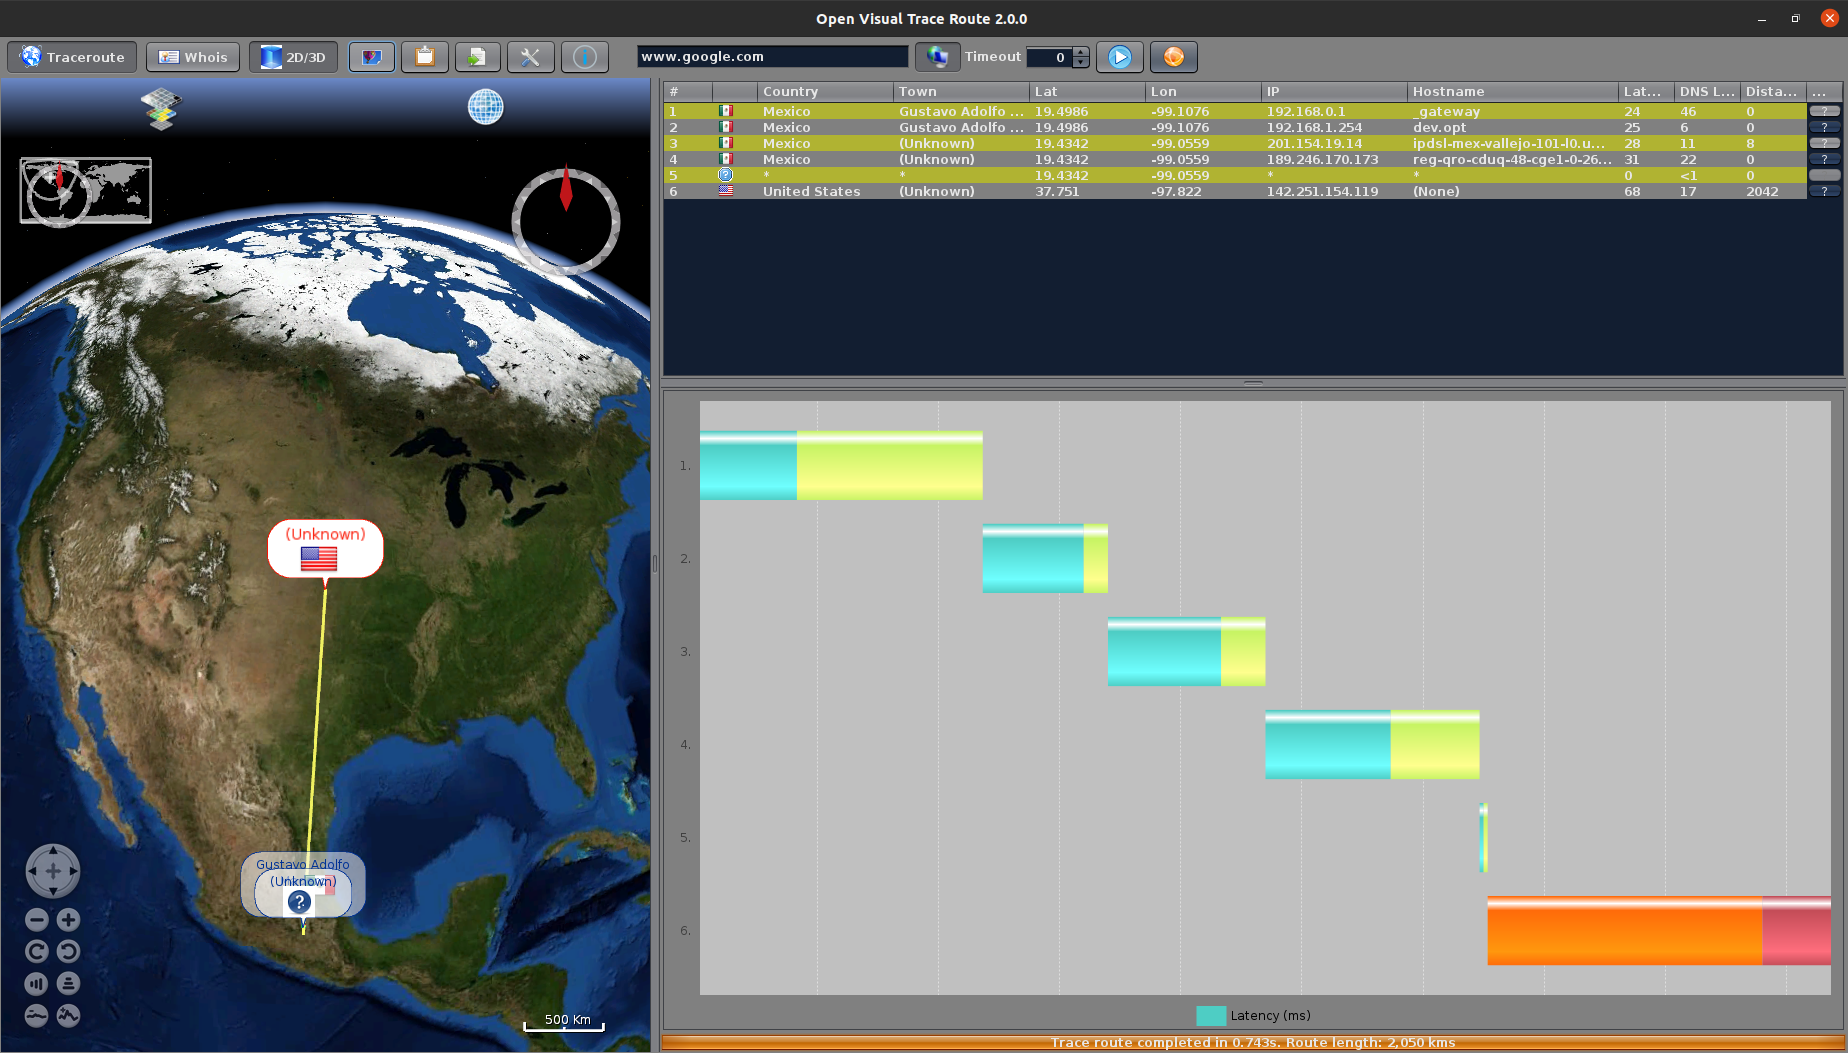
\includegraphics[width=0.9\textwidth]{image/imagen1Google.png}
        \caption{Rastreo de ruta hacia www.google.com (6 saltos, 0.743s).}
        \label{fig:google}
    \end{figure}

    \item \textbf{Destino: www.youtube.com}

    El ruteo hacia YouTube (resolviendo a la IP destino 192.178.56.174) muestra un comportamiento similar, predecible dado que también forma parte de la infraestructura masiva de Alphabet Inc. El trazado se completó con éxito en 10 saltos y un tiempo total de 0.668 segundos para una ruta de 2,050 kms. Aunque toma algunos saltos adicionales de enrutamiento en servidores intermedios de EE. UU. (como la IP \texttt{172.253.50.252}), la latencia final se mantiene excelente (43 ms), canalizando el tráfico de manera eficiente.

    \begin{figure}[H]
        \centering
        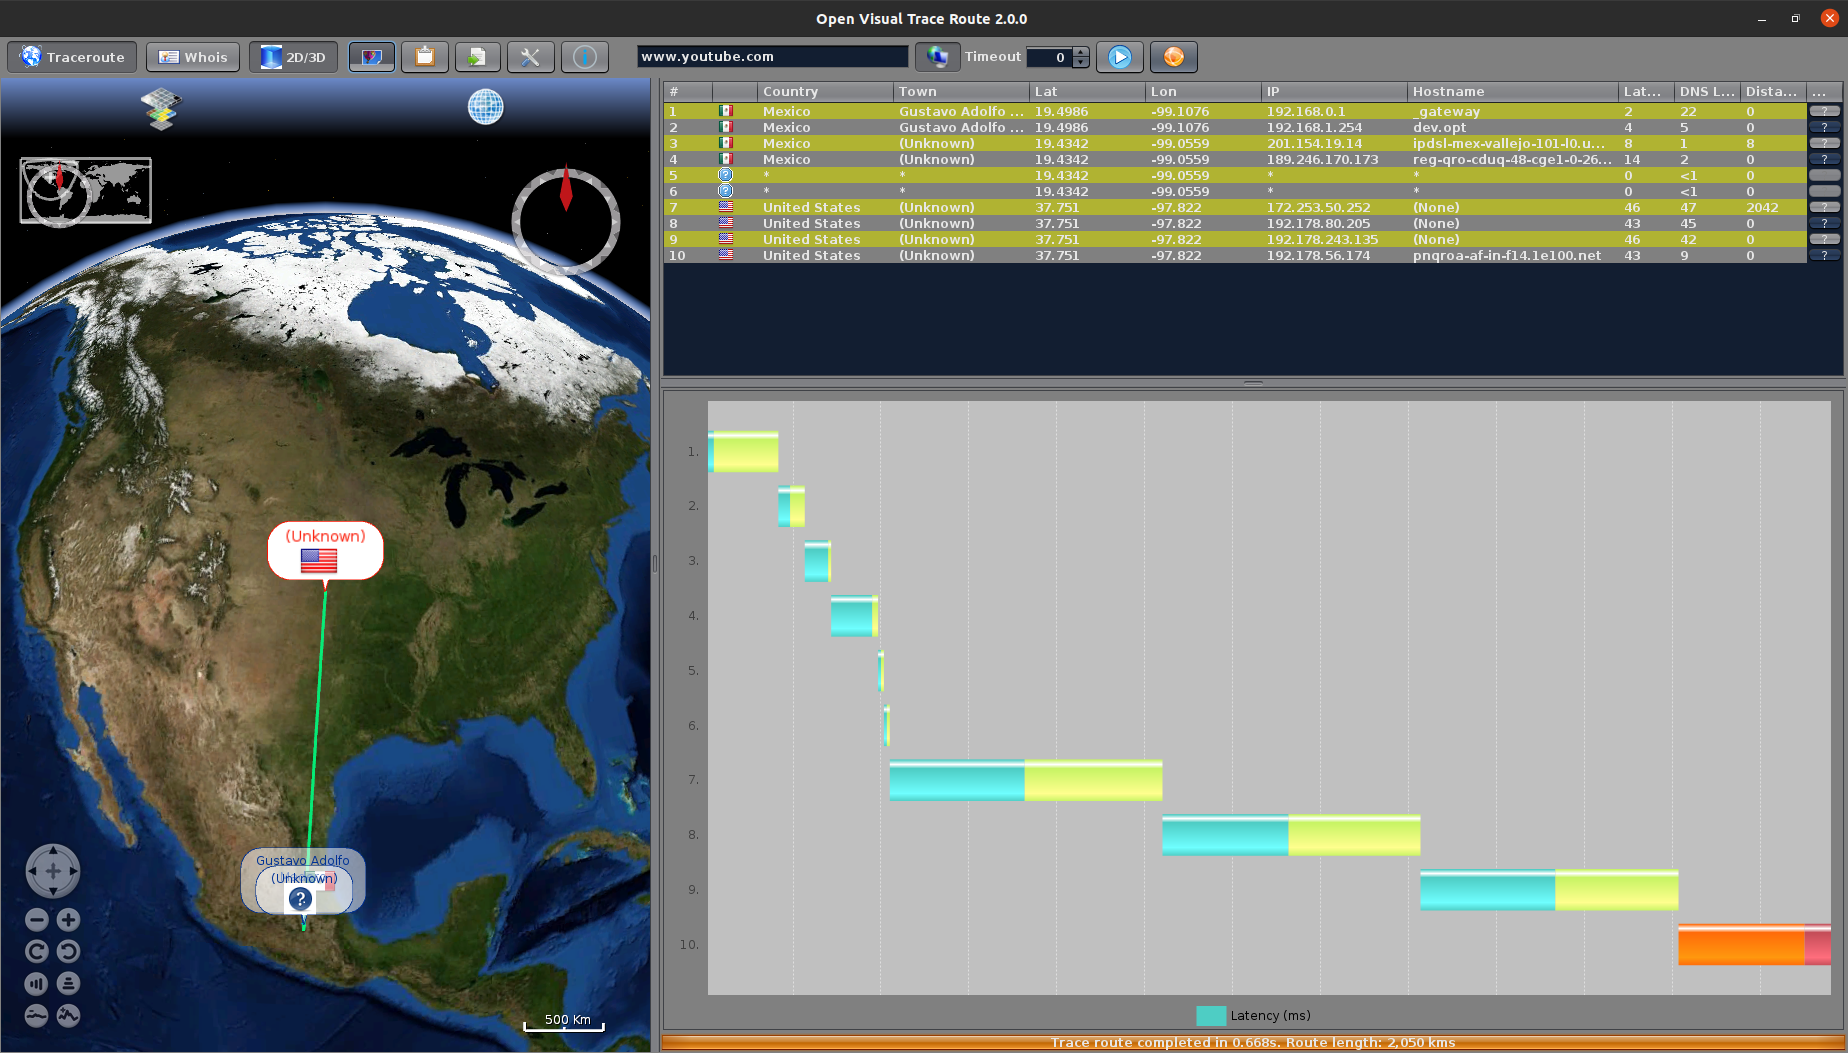
\includegraphics[width=0.9\textwidth]{image/imagen2youtube.png}
        \caption{Rastreo de ruta hacia www.youtube.com (10 saltos, 0.668s).}
        \label{fig:youtube}
    \end{figure}

    \item \textbf{Destino: wikipedia.com}

    El análisis hacia Wikipedia revela una topología donde el tráfico es enrutado a través de enlaces internacionales de mayor distancia. En el salto 6, el paquete llega a Dallas, Texas (IP \texttt{4.36.175.161}, perteneciente a redes de tránsito) y posteriormente al salto 7 (\texttt{4.69.210.137}). A partir del salto 8, el software marca la ruta con tiempos de espera hasta alcanzar el límite máximo de 50 saltos (``Trace route incomplete''). Este es un comportamiento común provocado por cortafuegos (firewalls) perimetrales que bloquean silenciosamente los paquetes de sondeo ICMP.

    \begin{figure}[H]
        \centering
        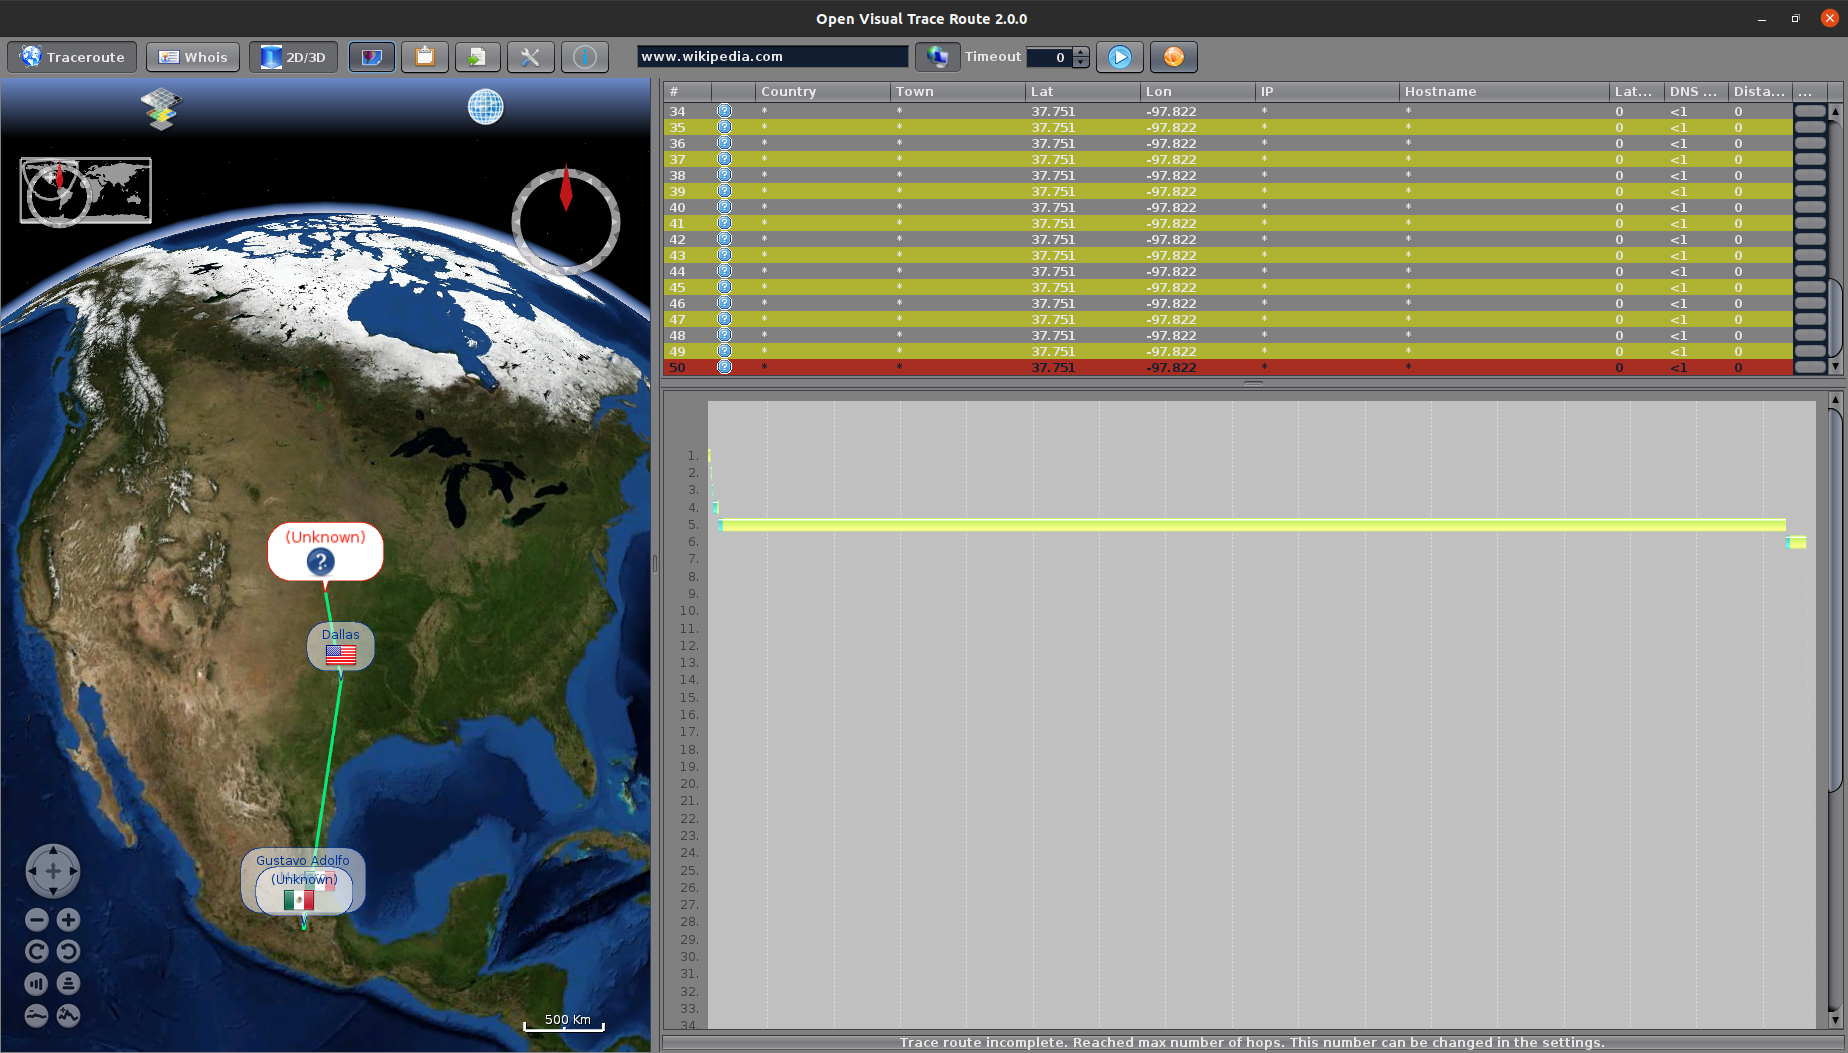
\includegraphics[width=0.9\textwidth]{image/imagen3wikipedia.png}
        \caption{Rastreo de ruta hacia wikipedia.com mostrando los primeros saltos hacia Dallas.}
        \label{fig:wiki1}
    \end{figure}

    \begin{figure}[H]
        \centering
        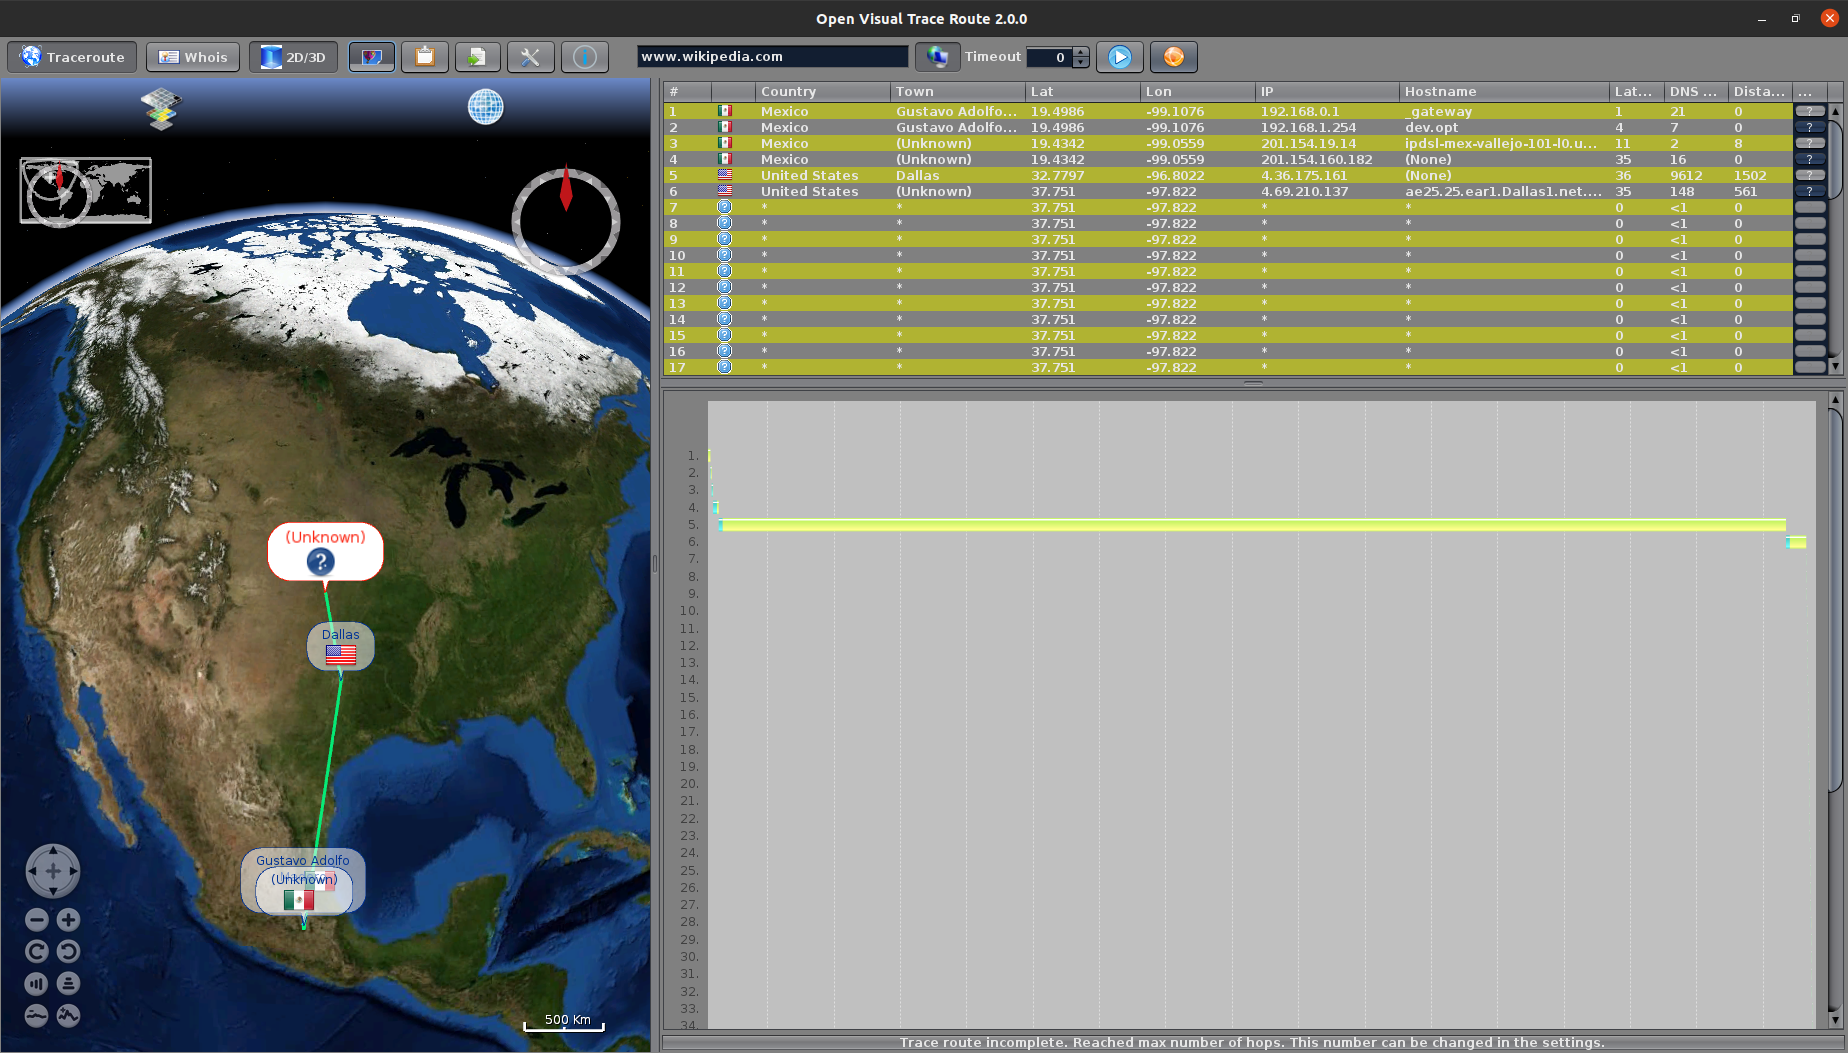
\includegraphics[width=0.9\textwidth]{image/imagen4wikipedia2.png}
        \caption{Continuación del rastreo hacia wikipedia.com (Límite de 50 saltos alcanzado).}
        \label{fig:wiki2}
    \end{figure}

    \item \textbf{Destino alternativo: seguridad.fi-b.unam.mx/Lab/index.php}

    Como enlace de preferencia se analizó un servidor alojado en la red de la Universidad Nacional Autónoma de México. El mapa 3D dibuja un recorrido que salta por nodos de proveedores nacionales: inicia en Gustavo A. Madero, pasa por Taxco (salto 5, \texttt{187.228.21.253}), Tijuana (salto 6, \texttt{189.204.203.101}) y Coyoacán (salto 9, \texttt{132.248.133.22}) antes de registrar actividad en la red de la UNAM (salto 10, IP \texttt{132.247.237.102}). A partir del salto 11, se registran tiempos de espera continuos hasta el salto 50, evidenciando las estrictas políticas de Listas de Control de Acceso (ACLs) perimetrales de la Facultad de Ingeniería.

    \begin{figure}[H]
        \centering
        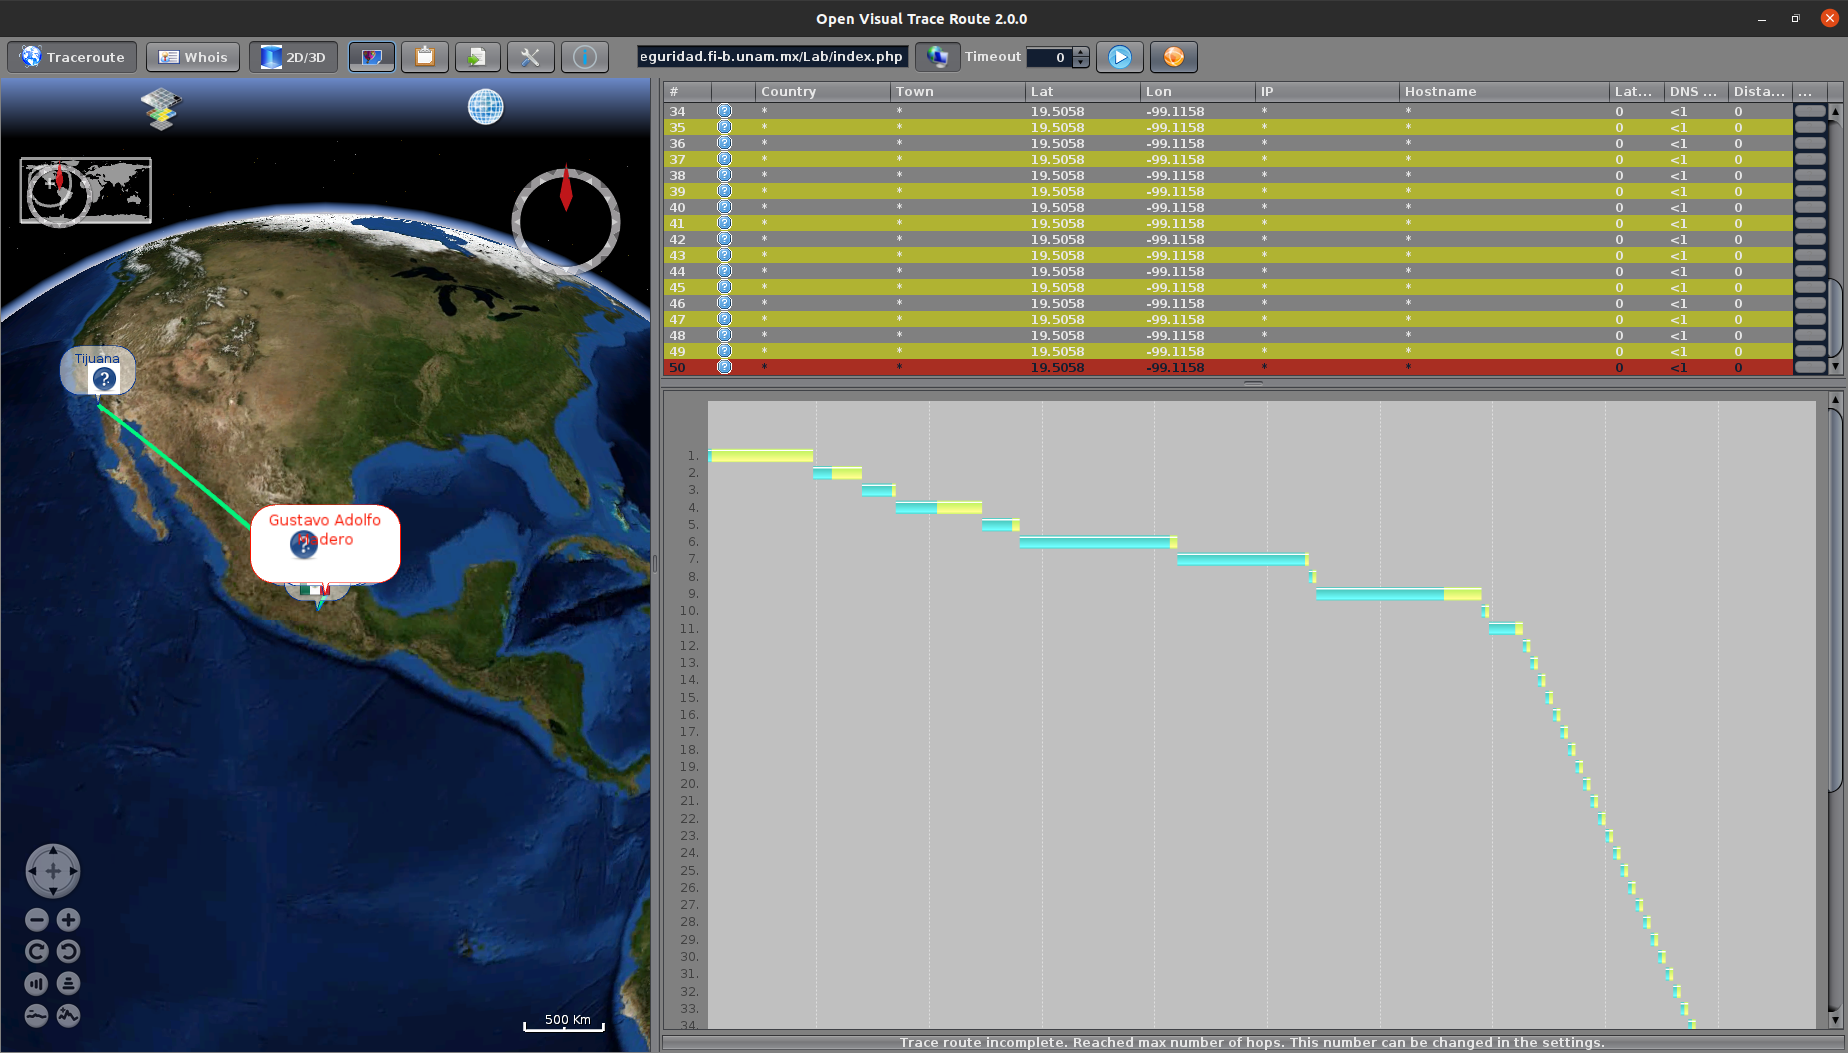
\includegraphics[width=0.9\textwidth]{image/imgen5labredes1.png}
        \caption{Rastreo de ruta hacia el servidor del Laboratorio de Redes Seguras.}
        \label{fig:unam1}
    \end{figure}

    \begin{figure}[H]
        \centering
        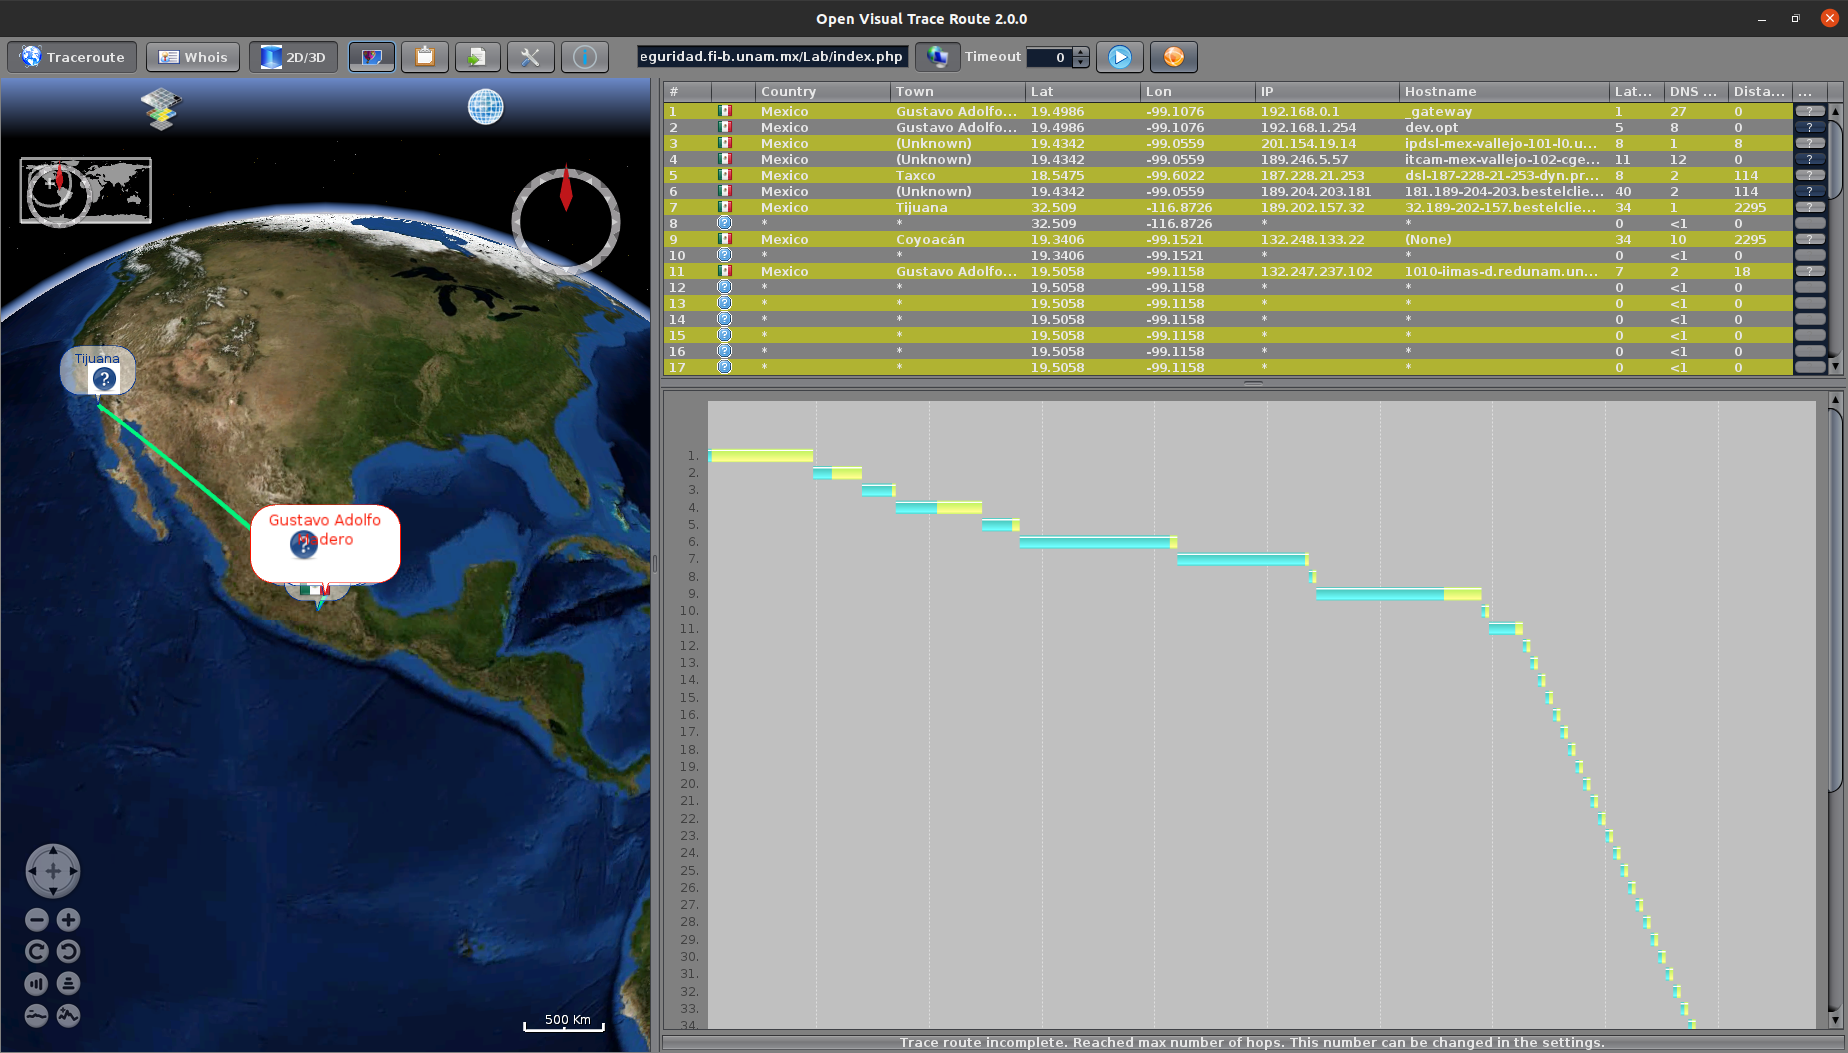
\includegraphics[width=0.9\textwidth]{image/imagen6labredes2.png}
        \caption{Continuación del rastreo hacia la UNAM mostrando políticas de bloqueo ICMP.}
        \label{fig:unam2}
    \end{figure}

\end{enumerate}


\newpage
\begin{thebibliography}{99}

\bibitem{ibm_ipv4_capa3} 
IBM Corp. (2025). \textit{Protocolos a nivel de red Internet: Protocolo Internet (IP)}. Documentación Técnica del Sistema Operativo AIX. Recuperado de la base de conocimientos IBM Docs.

\bibitem{cisco_ethernet_frames} 
Cisco Systems Inc. (2020). \textit{Campos de la trama Ethernet II y Encapsulamiento de Enlace de Datos}. Material de Estudio del Módulo 5, Certificación CCNA Routing \& Switching. Cisco Networking Academy.

\bibitem{cloudflare_osi_layer} 
Cloudflare, Inc. (2025). \textit{¿Qué es el modelo OSI? Definición de las 7 capas de interconexión y flujos de datos para mitigación DDoS}. Centro de Recursos y Aprendizaje TheNET.

\bibitem{ietf_rfc791} 
Internet Engineering Task Force (IETF). (1981). \textit{RFC 791: Protocolo de Internet (Internet Protocol) Especificación del Programa DARPA de Internet}. Editor de Peticiones de Comentarios de la Red.

\bibitem{aws_routing_concepts} 
Amazon Web Services, Inc. (2025). \textit{¿Qué es el enrutamiento? Conceptos de Reenvío de Datos y Algoritmos de encaminamiento en la Nube}. Guía Arquitectónica de Conceptos Fundamentales AWS.

\bibitem{redhat_tcpdump} 
Red Hat, Inc. (2024). \textit{Introducción al uso de tcpdump en la línea de comandos de Linux para resolución de problemas de red}. Blog de Recursos para Administradores de Sistemas Linux.

\bibitem{fortinet_arp_security} 
Fortinet, Inc. (2025). \textit{¿Qué es el Protocolo de Resolución de Direcciones (ARP)? Glosario de Seguridad Cibernética y Vectores de Envenenamiento ARP}. Repositorio de Amenazas Globales.

\bibitem{ionos_ethernet} 
IONOS SE. (2023). \textit{Trama Ethernet: definición, estructura y variantes (Ethernet II y IEEE 802.3)}. Digital Guide y Know-How para Servidores.

\bibitem{cisco_packet_tracer} 
Cisco Systems Inc. (2025). \textit{Cisco Packet Tracer: Software de simulación de redes y herramientas analíticas para entornos formativos y corporativos}. Repositorio y Knowledge Base Oficial de Cisco Learning Network.

\end{thebibliography}

\end{document}